% Created 2015-11-16 星期一 18:43
\documentclass{beamer}
\usepackage{fixltx2e}
\usepackage{graphicx}
\usepackage{longtable}
\usepackage{float}
\usepackage{wrapfig}
\usepackage{soul}
\usepackage{textcomp}
\usepackage{marvosym}
\usepackage{wasysym}
\usepackage{latexsym}
\usepackage{amssymb}
\usepackage{hyperref}
\tolerance=1000
\usepackage{etex}
\usepackage{amsmath}
\usepackage[usenames]{color}
\usepackage[all]{xy}
\usepackage{pstricks}
\usepackage{pgfplots}
\usepackage{tikz}
\usepackage[europeanresistors,americaninductors]{circuitikz}
\usepackage{colortbl}
\usepackage{yfonts}
\usetikzlibrary{shapes,arrows}
\usetikzlibrary{positioning}
\usetikzlibrary{arrows,shapes}
\usetikzlibrary{intersections}
\usetikzlibrary{calc,patterns,decorations.pathmorphing,decorations.markings}
\usepackage[BoldFont,SlantFont,CJKchecksingle]{xeCJK}
\setCJKmainfont[BoldFont=Evermore Hei]{Evermore Kai}
\setCJKmonofont{Evermore Kai}
\usepackage{pst-node}
\usepackage{pst-plot}
\psset{unit=5mm}
\usepackage{beamerarticle}
\mode<beamer>{\usetheme{Frankfurt}}
\mode<beamer>{\usecolortheme{dove}}
\mode<article>{\hypersetup{colorlinks=true,pdfborder={0 0 0}}}
\AtBeginSection[]{\begin{frame}<beamer>\frametitle{Topic}\tableofcontents[currentsection]\end{frame}}
\setbeamercovered{transparent}
\providecommand{\alert}[1]{\textbf{#1}}

\title{补充例子}
\author{}
\date{}
\hypersetup{
  pdfkeywords={},
  pdfsubject={},
  pdfcreator={Emacs Org-mode version 7.9.3f}}

\begin{document}

\maketitle

\begin{frame}
\frametitle{Outline}
\setcounter{tocdepth}{3}
\tableofcontents
\end{frame}









\begin{center}
\newcommand{\p}{*+[Fo]{} \ar[r]}
\newcommand{\g}{*+[F]{\frac{1}{s}} \ar[rr]}
\newcommand{\d}{*-<0em>{}\ar '[d]'[dll][ll]^<(0.7){-}}
\newcommand{\o}{*-<0em>{}}
  \xymatrix{
  R(s) \ar[r] & {\p} & {\g} &  {\d} & C(s) \\
              & {\o} &    &{\o}   &
  }
\end{center}



\section{关于反馈}
\label{sec-1}
\begin{frame}
\frametitle{反馈与方程(静态)}
\label{sec-1-1}


\begin{tikzpicture}[node distance=2em,auto,>=latex', thick]
%\path[use as bounding box] (-1,0) rectangle (10,-2); 
\path[->] node[] (r) {A}; 
\path[->] node[ circle,inner sep=2pt,minimum size=1pt,draw,label=below left:$ $,right =of r] (p1) { }; 
\path[->](r) edge node {} (p1) ; 
\path[red] node[draw, inner sep=5pt,right =of p1] (g) {$\frac{1}{3}$}; 
\path[->] (p1) edge node[midway] {B} (g) ; 
\path[->] node[ right =of g] (o) {C}; 
\path[->] (g) edge node {} (o); 
\path[blue] node[draw, below =of g] (h) {1};
\path[->,draw] (g.east)+(1em,0) |- (h.east) ; 
\path[->,draw] (h.west) -| (p1) ; 
\end{tikzpicture} 

\begin{eqnarray}
C &=& \frac{B}{3}\\
A+C &=& B\\
A &=& 10\\
C &=& ?
\end{eqnarray}
\end{frame}
\begin{frame}
\frametitle{笑话:过桥}
\label{sec-1-2}


路人甲要过桥,发现桥很长,问桥边路人乙桥长多少,乙说:50米。甲走上桥后不一会儿,乙追了上来,说,桥长100米,你要是过了50米就转弯,就掉下去了。

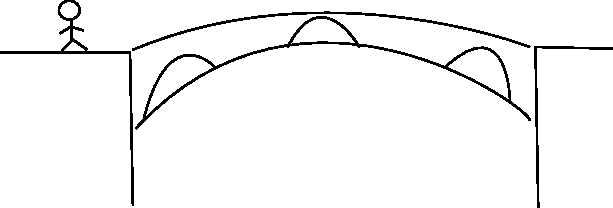
\includegraphics[width=\textwidth]{image/bridge.pdf}
\end{frame}
\begin{frame}
\frametitle{开环控制:笑话:不听话的儿子}
\label{sec-1-3}
\end{frame}
\begin{frame}
\frametitle{开环控制:声东击西}
\label{sec-1-4}
\end{frame}
\begin{frame}
\frametitle{操纵杆}
\label{sec-1-5}


飞行员拉动操纵杆,飞机机头上扬,结果减弱了拉动操纵杆的效果,即:拉杆->A增大->机头上扬->A减小

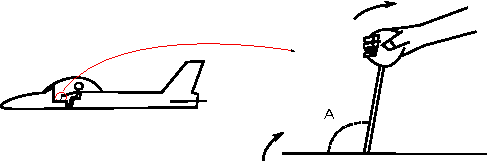
\includegraphics[width=\textwidth]{image/pilot.pdf}
\end{frame}
\begin{frame}
\frametitle{油门、刹车}
\label{sec-1-6}


司机踩刹车,汽车减速,司机因为惯性会有前冲的趋势,易导致踩刹车的力度变大。

司机踩油门,汽车加速,司机因为惯性会有后仰的趋势,易导致踩油门的力度变小。

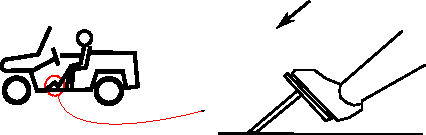
\includegraphics[width=\textwidth]{image/drive.pdf}
\end{frame}
\section{非线性}
\label{sec-2}
\begin{frame}
\frametitle{几个例子}
\label{sec-2-1}

\begin{align*}
c &= u\\
c &= u+1\\
c &= 1\\
c &= 0\\
c &= \sqrt[3]{u} \quad u= x^3 \\
c+c^2 &= u \quad u=r+c^{2}
\end{align*}
\end{frame}
\begin{frame}
\frametitle{$x'+1 =u$}
\label{sec-2-2}
\begin{columns}
\begin{column}{0.5\textwidth}
\begin{block}{方法1}
\label{sec-2-2-1}

变量代换,为方程右边与输出变量无关的部分指定另一个变量。
\begin{align*}
x'+1 &= u \\
w &= u-1 \\
x' &= w 
\end{align*}
\end{block}
\end{column}
\begin{column}{0.5\textwidth}
\begin{block}{方法2}
\label{sec-2-2-2}

将方程右边与输出变量无关的部分用泰勒级数展开。
\begin{align*}
x' &=u-1 \\
u-1 &= (u-1)|_{u=1}+\Delta u \\
x' &= \Delta u 
\end{align*}
\end{block}
\end{column}
\end{columns}
\end{frame}
\begin{frame}
\frametitle{$cc'=u$}
\label{sec-2-3}
\begin{columns}
\begin{column}{0.5\textwidth}
\begin{block}{在 $c_0=1,c'_0=1$ 处线性化}
\label{sec-2-3-1}


\begin{align*}
(1+\Delta c)(1+\Delta c') &= u \\
1+\Delta c+ \Delta c' + \Delta c \Delta c' &= u\\
\Delta c +\Delta c' &= \Delta u
\end{align*}
$\Delta u=0,u=1$ 时, $cc'=1$ 。接着随着 $c$ 增大,$c'$ 会减小。
\end{block}
\end{column}
\begin{column}{0.5\textwidth}
\begin{block}{变量代换 $c=t+\Delta c,c'=1+\Delta c'$}
\label{sec-2-3-2}

\begin{align*}
(t+\Delta c)(1+\Delta c') &=u \\
t+\Delta c+t\Delta c'+\Delta c\Delta c' &=u \\
\Delta c +t\Delta c' &= \Delta u
\end{align*}
$\Delta u=0,u=t$ 时, $cc'=t$ 。接着随着 $c$ 增大,$c'$ 不变。
\end{block}
\end{column}
\end{columns}
\end{frame}
\section{稳定性}
\label{sec-3}
\begin{frame}
\frametitle{稳定性与平衡点}
\label{sec-3-1}


\begin{eqnarray*}
\dot x(t)-x(t) & = & r(t)\\
r &=& 1 \\
x(0) &=& -1 \\
x(t) &=& -1
\end{eqnarray*}

\begin{itemize}
\item 通解:$x_1(t)=a_0e^t$
\item 特解:$x_2(t)=-1$
\item $x_1(0)+x_2(0)=x(0)$得$a_0=0$
\end{itemize}
\end{frame}
\begin{frame}
\frametitle{正反馈与离散系统稳定性}
\label{sec-3-2}

\begin{eqnarray*}
x(n+1)-kx(n) &=& r(n) \\
r(n) & = & 0 \\
x(n) &=& x(0)k^n
\end{eqnarray*}
\end{frame}
\begin{frame}
\frametitle{正反馈与延迟系统稳定性}
\label{sec-3-3}

\begin{eqnarray*}
x(t+a)-kx(t) &=& r(t) \\
r(t) &=& 0 \\
x(na) &=& x(0)k^{n}
\end{eqnarray*}
\end{frame}
\section{卷积}
\label{sec-4}
\begin{frame}
\frametitle{卷积与脉冲响应}
\label{sec-4-1}

\begin{itemize}
\item 卷积
      \begin{eqnarray*}
      x(t)*y(t) &=& \int_{-\infty}^{\infty}x(\tau)y(t-\tau)d\tau \\
      x(t)*\delta(t)& = & x(t) \\
      \end{eqnarray*}
\item 脉冲响应
     设线性时不变(Linear Time Invariant,LTI)系统脉冲响应为 $h(t)$ :
      \begin{eqnarray*}
      h(t) &=& LTI[\delta(t)]\\
      h(t-\tau) &=& LTI[\delta(t-\tau)]\\
      \end{eqnarray*}
\end{itemize}
\end{frame}
\begin{frame}
\frametitle{卷积与系统响应}
\label{sec-4-2}

设输入信号为 $x(t)$ 时,输出为 $y(t)$ :
\begin{eqnarray*}
y(t) & =& LTI[x(t)]\\
     &=& LTI\left[\int_{-\infty}^{\infty}x(\tau)\delta(t-\tau)d\tau\right] \\
     &=& \int_{-\infty}^{\infty} LTI[x(\tau)\delta(t-\tau)]d\tau \\
     &=& \int_{-\infty}^{\infty} x(\tau)LTI[\delta(t-\tau)]d\tau \\
     &=& \int_{-\infty}^{\infty} x(\tau) h(t-\tau)d\tau \\
     &=& x(t) * h(t)
\end{eqnarray*}
\end{frame}
\section{误差}
\label{sec-5}
\begin{frame}
\frametitle{阶跃输入}
\label{sec-5-1}


\begin{eqnarray*}
 m \dot{v} & =& f\\
 m \dot{v} & =& r-v\\
 m \dot{v} & =& 1-v\\
 m \frac{d}{dt}(v-1) & =& 1-v\\
 m \frac{d}{dt}(1-v) & =& -(1-v)\\
m \dot{E} &=& -E \\
E &=& e^{-\frac{t}{m}}
\end{eqnarray*}
\end{frame}
\begin{frame}
\frametitle{斜坡输入}
\label{sec-5-2}


\begin{eqnarray*}
 m \dot{v} & =& f\\
 m \dot{v} & =& r-v\\
 m \dot{v} & =& t-v\\
 m \frac{d}{dt}{v-t} +m & =& t-v\\
 m \frac{d}{dt}{t-v} & =& -(t-v) +m\\
m \dot{E} &=& -E +m\\
E &=& (1-m)e^{-\frac{t}{m}}+m
\end{eqnarray*}
\end{frame}
\section{Fourier变换}
\label{sec-6}
\begin{frame}
\frametitle{Fourier级数(三角形式)}
\label{sec-6-1}

\begin{eqnarray*}
f_T(t) & =& \frac{a_0}{2}+\sum_{n=1}^{\infty}(a_n\cos(n\omega t)+b_n\sin(n\omega t))  
\end{eqnarray*}
其中:
\begin{eqnarray*}
\omega & =& \frac{2\pi}{T}\\
a_0 &=& \frac{2}{T}\int_{-\frac{T}{2}}^{\frac{T}{2}}f_T(t)dt \\
a_n &=& \frac{2}{T}\int_{-\frac{T}{2}}^{\frac{T}{2}}f_T(t)\cos(n\omega t)dt \\
b_n &=& \frac{2}{T}\int_{-\frac{T}{2}}^{\frac{T}{2}}f_T(t)\sin(n\omega t)dt \\
\end{eqnarray*}
\end{frame}
\begin{frame}
\frametitle{Fourier级数(复指数形式)}
\label{sec-6-2}

\begin{eqnarray*}
f_T(t) & = & \sum_{n=-\infty}^{+ \infty}c_n e^{j\omega_n t} \\
f_T(t) & = & \frac{1}{T}\sum_{n=-\infty}^{+\infty}\left[ \int_{- \frac{T}{2} }^{\frac{T}{2}}f_T(\tau)e^{-j\omega_n\tau}d\tau\right] e^{j\omega_n t} 
\end{eqnarray*}
\end{frame}
\begin{frame}
\frametitle{Fourier积分}
\label{sec-6-3}

\begin{eqnarray*}
\lim_{T\rightarrow+\infty}f_T(t) &=& f(t) \\
f(t) & = & \lim_{T\rightarrow+\infty}\frac{1}{T}\sum_{n=-\infty}^{+\infty}\left[ \int_{- \frac{T}{2} }^{\frac{T}{2}}f_T(\tau)e^{-j\omega_n\tau}d\tau\right] e^{j\omega_n t} \\
\Delta\omega &=& \frac{2\pi}{T} \\
f(t) & = & \lim_{\Delta\omega\rightarrow 0}\frac{1}{2\pi}\sum_{n=-\infty}^{+ \infty}\left[ \int_{- \frac{T}{2} }^{\frac{T}{2}}f_T(\tau)e^{-j\omega_n\tau}d\tau\right] e^{j\omega_n t}\Delta\omega \\
f(t) & = & \frac{1}{2\pi}\int_{-\infty}^{+\infty}\left[ \int_{-\infty }^{\infty}f(\tau)e^{-j\omega_n\tau}d\tau\right] e^{j\omega_n t}d\omega
\end{eqnarray*}
\end{frame}
\begin{frame}
\frametitle{Fourier变换定义}
\label{sec-6-4}

\begin{eqnarray*}
f(t)& = &\frac{1}{2\pi}\int_{-\infty}^{+\infty}\left[ \int_{-\infty }^{\infty}f(\tau)e^{-j\omega_n\tau}d\tau\right]e^{j\omega_n t}d\omega \\
F(j\omega)&=& \int_{-\infty}^{ + \infty}f(t)e^{-j\omega t}dt \\
f(t)  & =& \frac{1}{2\pi} \int_{-\infty}^{+\infty}F(j\omega)e^{j\omega t}d\omega \\
F(j\omega) &=& {\cal F}[f(t)] \\
f(t) &=& {\cal F}^{-1}[F(j\omega)] 
\end{eqnarray*}
\end{frame}
\begin{frame}
\frametitle{常用函数的Fourier变换}
\label{sec-6-5}

\begin{itemize}
\item 单位脉冲函数 $f(t)=\delta(t) \rightarrow   F(j\omega)=1$
\item 阶跃函数 $f(t)=A,(t\geq 0) \rightarrow   F(j\omega)=\pi\delta(\omega)+\frac{1}{j\omega}$
\item 指数函数 $f(t)=e^{at},(t\geq 0) \rightarrow  F(j\omega)=\frac{1}{j\omega-a}$
\item 正弦函数 $f(t)=\sin(\omega_0 t)\rightarrow F(j\omega)=\pi[\delta(\omega+\omega_0)+\delta(\omega-\omega_0)]$
\end{itemize}
\end{frame}
\begin{frame}
\frametitle{性质}
\label{sec-6-6}

\begin{itemize}
\item 线性: $f(t)=af_1(t)+bf_2(t)\rightarrow  F(j\omega)=aF_1(j\omega)+bF_2(j\omega)$,其中 $a,b$ 为常数
\item 时移: $g(t)=f(t\pm a) \rightarrow  G(s)=F(j\omega)e^{\pm j\omega a}$
\item 频移:${\cal F}[e^{\pm\omega_0 t}f(t)]=F(j(\omega\mp\omega_0))$
\item 时域微分: $g(t)=f(t)'\rightarrow  G(j\omega)=j\omega F(j\omega)$
\item 频域微分:${\cal F}[tf(t)]=j\frac{dF(j\omega)}{d\omega}$
\item 时域积分: $g(t)=\int_{-\infty}^{t} f(\tau) d\tau \rightarrow  G(j\omega)=\frac{F(j\omega)}{j\omega}+\pi F(0)\delta(\omega)$
\item 卷积:${\cal F}[f_1(t)*f_2(t)]={\cal F}[f_1(t)]{\cal F}[f_2(t)]$
\end{itemize}
\end{frame}
\section{连续系统频域分析}
\label{sec-7}
\begin{frame}
\frametitle{基本信号 $e^{j\omega t}$ 通过线性系统}
\label{sec-7-1}

\begin{eqnarray*}
f(t) & =& e^{j\omega t},\qquad -\infty < t < \infty \\
H(j\omega) &=& \int_{-\infty}^{\infty}h(t)e^{-j\omega t}dt \\
           &=& |H(j\omega)|e^{j\phi(\omega)} \\
y_f(t) &=& e^{j\omega t}*h(t) \\
       &=& \int_{-\infty}^{\infty}h(\tau)e^{j\omega(t-\tau)}d\tau \\
       &=& e^{j\omega t}\int_{-\infty}^{\infty}h(\tau)e^{-j\omega t}d\tau \\
       &=& H(j\omega)e^{j\omega t} \\
       &=& |H(j\omega)|e^{j(\omega t+\phi(\omega))}
\end{eqnarray*}
\end{frame}
\begin{frame}
\frametitle{正弦(余弦)信号通过线性系统}
\label{sec-7-2}

\begin{eqnarray*}
f(t) & =& A\cos\omega t , \qquad  -\infty<t<\infty \\
     &=&\frac{A}{2}(e^{j\omega t}+e^{-j\omega t}) \\
y_f(t) &=& \frac{A}{2}(H(j\omega)e^{j\omega t}+H(-j\omega)e^{-j\omega t}) \\
       &=& \frac{A}{2}|H(j\omega)|(e^{j\omega t+\phi(\omega)}+e^{-j\omega t-\phi(\omega)}) \\
       &=& A|H(j\omega)|\cos(\omega t+\phi(\omega)) \\
\end{eqnarray*}
\end{frame}
\begin{frame}
\frametitle{非正弦周期信号通过线性系统}
\label{sec-7-3}

\begin{eqnarray*}
f(t) &=& \sum_{n=-\infty}^{\infty}F_n e^{jn\omega t} \\
F_n &=& \frac{1}{T}\int_{-\frac{T}{2}}^{\frac{T}{2}}f(t)e^{-jn\omega t}dt \\
    &=& |F_n|e^{j\theta(n\omega)} \\
y_f(t) &=& \sum_{n=-\infty}^{\infty}F_nH(jn\omega)e^{jn\omega t} \\
       &=& \sum_{n=-\infty}^{\infty}|F_n||H(jn\omega)|e^{jn\omega t+\phi(n\omega)+\theta(n\omega)} \\
       &=& F_0+ \sum_{n=-\infty}^{\infty}2|F_n||H(jn\omega)|\cos(jn\omega t+\phi(n\omega)+\theta(n\omega))
\end{eqnarray*}
\end{frame}
\begin{frame}
\frametitle{系统对非周期信号的响应}
\label{sec-7-4}

\begin{eqnarray*}
y(t) & =& f(t)*h(t)\\
Y(j\omega) &=& F(j\omega)H(j\omega)\\
y(t) &=& {\cal F}^{-1}[Y(j\omega)] \\
H(j\omega) &=& \frac{Y(j\omega)}{F(j\omega)}
\end{eqnarray*}
\end{frame}
\begin{frame}
\frametitle{利用Fourier变换计算零状态响应}
\label{sec-7-5}

某线性时不变系统的脉冲响应 $h(t)=(e^{-2t}-e^{-3t})U(t)$ ,求输入信号 $f(t)=e^{-t}U(t)$ 时系统的零状态响应。其中 $U(t)$ 为单位阶跃函数。

解:

\begin{eqnarray*}
F(j\omega) & =& {\cal F}[f(t)] = \frac{1}{j\omega+1} \\ H(j\omega) &=& {\cal F}[h(t)] = \frac{1}{j\omega+2}-\frac{1}{j\omega+3}=\frac{1}{(j\omega+2)(j\omega+3)}\\
Y(j\omega) &=& F(j\omega)H(j\omega) = \frac{1}{(j\omega+1)(j\omega+2)(j\omega+3)}\\
           &=& \frac{1/2}{j\omega+1}+\frac{-1}{j\omega+2}+\frac{1/2}{j\omega+3}\\
y(t) &=& (\frac{1}{2}e^{-t}-e^{-2t}+\frac{1}{2}e^{-3t})U(t)
\end{eqnarray*}
\end{frame}
\section{部分分式分解求解差分方程}
\label{sec-8}
\begin{frame}
\frametitle{$C(n+2)-6C(n+2)+8C(n)=U(n)$ 零状态阶跃响应}
\label{sec-8-1}

部分分式分解方法有两种,求和限不同,但结果相同。
\begin{align*}
(z^2-6z+8)C(z)&=\frac{z}{z-1} \\
C(z) &= \frac{z}{(z-1)(z-2)(z-4)}\\
C(z) &=\frac{1}{3(z-1)}-\frac{1}{z-2}+\frac{2}{3(z-4)} \\
 &=\sum_{n=1}^{\infty}[\frac{1}{3}z^{-n}-\frac{1}{2}2^n z^{-n}+\frac{1}{6}4^n z^{-n}] \\
C(z) &=\frac{z}{3(z-1)}-\frac{z}{2(z-2)}+\frac{z}{6(z-4)}\\
 &=\sum_{n=0}^{\infty}[\frac{1}{3}z^{-n}-\frac{1}{2}2^n z^{-n}+\frac{1}{6}4^n z^{-n}] 
\end{align*}
\end{frame}
\begin{frame}
\frametitle{$C_{n+2}+3C_{n+1}+2C_{n}=0$ 求 $C(0)=0,C(1)=1$ 时的响应}
\label{sec-8-2}

部分分式分解有两种,可以看到,第一种分解计算时,如果 $n$ 的取值范围没有限定好,会出现错误。(如:求和时设定 $n$ 从1开始。)
\begin{align*}
& z^2C(z)-z^2+3(zC(z)-z)+2C(z)=0 \\
% (z^2+3z+2)C(z) &= z^2+3z \\
C(z) &= \frac{2}{z+2}-\frac{2}{z+1}+1 \\
     &= \sum_{n=1}^{\infty}[-(-2)^{n} z^{-n}]+\sum_{n=1}^{\infty}[2(-1)^n z^{-n}]+1 \\
     &= 1+0z^{-1}+\cdots \\
C(z) &=\frac{2z}{z+1}-\frac{z}{z+2} \\
     &=\sum_{n=0}^{\infty}[2(-1)^n z^{-n}]-\sum_{n=0}^{\infty}(-2)^n z^{-n}\\
C(n) &= 2(-1)^n-(-2)^n
\end{align*}
\end{frame}
\begin{frame}
\frametitle{两种部分分式分解之间的关系}
\label{sec-8-3}

从上面的例子可以看出,两种部分分式都可以求解出差分方程的解,但一个能够直接利用z反变换求解出时域函数,另一个要用到z变换的性质 ${\cal Z}[e(t-T)]=E(z)z^{-1}$ 。因此,解的范围不同,一个是 $n\geq 0$ ,一个是 $n\geq 1$ 。这两个解中包含共同的项(对应于差分方程的特征根),它们在 $n\leq 1$ 时是一致的。由于第一种方法的解从 $n=1$ 开始求和,因此它们只是在 $n=0$ 时相差一个常数。而分析第二种方法的解,可以从其它部分推导出来。

对于n阶差分方程,知道通解、特解与初始条件即可惟一确定其解。而初始条件可以替换为任意n个时刻的值。当两个函数满足通解与特解条件,并且在两个时刻的值相等时,可以断定这两个函数相等,都是方程的解。
\end{frame}
\section{最少拍控制}
\label{sec-9}
\begin{frame}
\frametitle{最小拍}
\label{sec-9-1}

为使误差信号在有限拍内变为0,设 $X(z)$ 为关于 $z^{-1}$ 的有限多项式:
\begin{align*}
\frac{1}{1+D(z)G(z)}\cdot\frac{A(z)}{(1-z^{-1})^m} &=A(z)X(z) \\
\frac{1}{1+D(z)G(z)} &=X(z){(1-z^{-1})^m} \\
D(z)G(z) &= \frac{1}{X(z)(1-z^{-1})^m}-1 \\
D(z) &= \frac{1-X(z)(1-z^{-1})^m}{X(z)(1-z^{-1})^m G(z)} 
\end{align*}
\end{frame}
\begin{frame}
\frametitle{无纹波最少拍}
\label{sec-9-2}

为使误差信号在有限拍内变为0,且控制器 $D(z)$ 的输出在有限拍内为常值,设 $X(z)$ 为关于 $z^{-1}$ 的有限多项式,$Y(z)$ 为关于 $z^{-1}$ 的有限多项式,或有一个极点 $z=1$ 
\begin{align*}
\frac{1}{1+D(z)G(z)}\cdot\frac{A(z)}{(1-z^{-1})^m} &=A(z)X(z) \\
\frac{D(z)}{1+D(z)G(z)}\cdot\frac{A(z)}{(1-z^{-1})^m} &=A(z)Y(z) \\
D(z) &= \frac{Y(z)}{X(z)}\\
(1+\frac{Y(z)}{X(z)}G(z))(1-z^{-1})^m &=\frac{1}{X(z)}\\
(X(z)+Y(z)G(z))(1-z^{-1})^m &=1\\
\end{align*}
\end{frame}
\begin{frame}[fragile]
\frametitle{无纹波最少拍示例}
\label{sec-9-3}

\begin{align*}
G(z) &=\frac{3.68z^{-1}(1+0.717z^{-1})}{(1-z^{-1})(1-0.368z^{-1})} \\
R(z) &=\frac{Tz^{-1}}{(1-z^{-1})^2} \\
X(z) &= 1+cz^{-1}\\
Y(z) &= \frac{(1-0.368z^{-1})(a+bz^{-1})}{1-z^{-1}}\\
b &=-0.22435314655638\\
c &=-0.59196923837781\\
a &=0.38261705478864
\end{align*}

\begin{verbatim}
e:3.68*z*(1+0.717*z)*(a+b*z)+(1-c*z)*(1-z)^2;
m:map(lambda([i],coeff((taylor(e,z,0,3)),z,i)),[1,2,3]);
float(solve(m));
\end{verbatim}
\end{frame}

\end{document}
